%allgemeine Formatangaben
\documentclass[
 a4paper, 										% Papierformat
 12pt,												% Schriftgröße
 ngerman, 										% für Umlaute, Silbentrennung etc.
 %titlepage,										% es wird eine Titelseite verwendet
 oneside, 										% einseitiges Dokument
 captions=nooneline,					% einzeilige Gleitobjekttitel ohne Sonderbehandlung wie mehrzeilige Gleitobjekttitel behandeln
 numbers=noenddot,						% Überschriften-??Nummerierung ohne Punkt am Ende
 parskip=half,									% zwischen Absätzen wird eine halbe Zeile eingefügt
 ]{scrartcl}

% Anpassung an Landessprache
\usepackage[ngerman]{babel}	

\usepackage[T1]{fontenc}	
\usepackage[utf8]{inputenc}	
\usepackage{textcomp} 																% Euro-Zeichen und andere
\usepackage[babel,german=quotes]{csquotes}						% Anführungszeichen
\RequirePackage[ngerman=ngerman-x-latest]{hyphsubst} 	% erweiterte Silbentrennung

% Befehle aus AMSTeX für mathematische Symbole z.B. \boldsymbol \mathbb
\usepackage{amsmath,amsfonts}

% Zeilenabstände und Seitenränder 
\usepackage{setspace}
\usepackage{geometry}

% Einbinden von JPG-Grafiken
\usepackage{graphicx}

% zum Umfließen von Bildern
% Verwendung unter http://de.wikibooks.org/wiki/LaTeX-Kompendium:_Baukastensystem#textumflossene_Bilder
\usepackage{floatflt}

% Verwendung von vordefinierten Farbnamen zur Colorierung
% Palette und Verwendung unter http://kitt.cl.uzh.ch/kitt/CLinZ.CH/src/Kurse/archiv/LaTeX-Kurs-Farben.pdf
\usepackage[usenames,dvipsnames]{color} 

% Tabellen
\usepackage{array}
\usepackage{longtable}

% einfache Grafiken im Code
% Einführung unter http://www.math.uni-rostock.de/~dittmer/bsp/pstricks-bsp.pdf
\usepackage{pstricks}

% Quellcodeansichten
\usepackage{verbatim}
\usepackage{moreverb} 											% für erweiterte Optionen der verbatim Umgebung
% Befehle und Beispiele unter http://www.ctex.org/documents/packages/verbatim/moreverb.pdf
\usepackage{listings}
\lstset{literate=
  {á}{{\'a}}1 {é}{{\'e}}1 {í}{{\'i}}1 {ó}{{\'o}}1 {ú}{{\'u}}1
  {Á}{{\'A}}1 {É}{{\'E}}1 {Í}{{\'I}}1 {Ó}{{\'O}}1 {Ú}{{\'U}}1
  {à}{{\`a}}1 {è}{{\`e}}1 {ì}{{\`i}}1 {ò}{{\`o}}1 {ù}{{\`u}}1
  {À}{{\`A}}1 {È}{{\'E}}1 {Ì}{{\`I}}1 {Ò}{{\`O}}1 {Ù}{{\`U}}1
  {ä}{{\"a}}1 {ë}{{\"e}}1 {ï}{{\"i}}1 {ö}{{\"o}}1 {ü}{{\"u}}1
  {Ä}{{\"A}}1 {Ë}{{\"E}}1 {Ï}{{\"I}}1 {Ö}{{\"O}}1 {Ü}{{\"U}}1
  {â}{{\^a}}1 {ê}{{\^e}}1 {î}{{\^i}}1 {ô}{{\^o}}1 {û}{{\^u}}1
  {Â}{{\^A}}1 {Ê}{{\^E}}1 {Î}{{\^I}}1 {Ô}{{\^O}}1 {Û}{{\^U}}1
  {œ}{{\oe}}1 {Œ}{{\OE}}1 {æ}{{\ae}}1 {Æ}{{\AE}}1 {ß}{{\ss}}1
  {ű}{{\H{u}}}1 {Ű}{{\H{U}}}1 {ő}{{\H{o}}}1 {Ő}{{\H{O}}}1
  {ç}{{\c c}}1 {Ç}{{\c C}}1 {ø}{{\o}}1 {å}{{\r a}}1 {Å}{{\r A}}1
  {€}{{\euro}}1 {£}{{\pounds}}1 {«}{{\guillemotleft}}1
  {»}{{\guillemotright}}1 {ñ}{{\~n}}1 {Ñ}{{\~N}}1 {¿}{{?`}}1
} 											% für angepasste Quellcodeansichten siehe
% Kurzeinführung unter http://blog.robert-kummer.de/2006/04/latex-quellcode-listing.html

\usepackage{pgfplots}
\usepackage{pgfplotstable}
\usepackage{filecontents}
\pgfplotsset{compat=1.9}

% verlinktes und Farblich angepasstes Inhaltsverzeichnis
\usepackage[pdftex,
colorlinks=true,
linkcolor=InterneLinkfarbe,
urlcolor=ExterneLinkfarbe]{hyperref}
\usepackage[all]{hypcap}

% URL verlinken, lange URLs umbrechen
\usepackage{url}

% sorgt dafür, dass Leerzeichen hinter parameterlosen Makros nicht als Makroendezeichen interpretiert werden
\usepackage{xspace}

% Beschriftungen für Abbildungen und Tabellen
\usepackage{caption}

% Entwicklerwarnmeldungen entfernen
\usepackage{scrhack}

\newcommand{\qq}[1]{\glqq{#1\grqq{}}} %Gänsefüßchen

\onehalfspacing 							% 1,5facher Zeilenabstand

\definecolor{InterneLinkfarbe}{rgb}{0.1,0.1,0.3} 	% Farbliche Absetzung von externen Links
\definecolor{ExterneLinkfarbe}{rgb}{0.1,0.1,0.7}	% Farbliche Absetzung von internen Links

% Einstellungen für Fußnoten:
\captionsetup{font=footnotesize,labelfont=sc,singlelinecheck=true,margin={5mm,5mm}}	
					
\title{Dokumentation zu den Projektaufgaben 1 und 2}
\subtitle{Message Passing Programmierung}

\author{Matthias Zober und Michael Horn\vspace{5cm}}
\date{\today}
\begin{document}

\maketitle
\tableofcontents
\thispagestyle{empty}
\pagebreak
\setcounter{page}{1}

\section{Überblick}
In dieser Dokumentation werden die Aufgaben \qq{Rechteckmustererkennung} sowie \qq{Numerische Integration mittels Parabelformel} betrachtet und hinsichtlich ihrer Parallelität untersucht.
Der entstandene Quellcode kann unter:\\
\url{https://github.com/MZober1993/MessagePassingProjects}\footnote{Letzter Aufruf: \today}
eingesehen werden.\\
Ebenfalls befinden sich in diesem Repository alle ermittelten Messwerte als CSV-Dateien sowie die erstellten Skripte zur Ermittlung der Laufzeiten.

\section{Projektaufgabe 1: Rechteckmustererkennung}
In diesem Abschnitt wird die Umsetzung der Projektaufgabe 1 dargestellt, die Verwendung erläutert sowie Laufzeitverhalten, Speedup und Effizienz untersucht. 
Außerdem erfolgt eine Auswertung am Ende dieses Abschnittes.
Das zu spezifizierende parallele Programm soll eine Rechteckmustererkennung für ein Digitalbild über ein Cluster realisieren.

\subsection{Realisierung}
\label{ref:realisierungRect}
Für die Umsetzung eines solchen Programms ist es zunächst notwendig eine sequentielle Erkennung eines $n*m$ Pixelbildes zu realisieren.
Für die Parallelisierung muss jeder Prozessor diese sequentielle Erkennung auf sein Teilbild anwenden. Hierzu ist es notwendig, dass nach dem Einlesen des Bildes durch 
einen ausgezeichneten Hauptprozess (\texttt{Master}), die resultierenden Teilbilder auf alle Prozesse verteilt werden. 
Diese Aufteilung wird im Programm durch \texttt{MPI\_Scatter} realisiert, durch diese Verteilung muss eine ungerade Prozessoranzahl ausgeschlossen werden.

Im Wesentlichen wird ein Rechteck durch das Finden eines schwarzen Pixels \linebreak(schwarz=0, weiß=1) und das Überprüfen von ausschließenden Mustern gefunden. 
Die Erkennung kann realisiert werden durch die Speicherung der Koordinaten des ersten (\texttt{startX} und \texttt{startY}) und zuletzt gefundenen Pixels (\texttt{stopX} und \texttt{stopY}) und die Länge der oberen gefunden Rechteckkante (\texttt{xSize}). Im folgenden erkennt man die ausschließenden Mustern mit deren Regeln.
\begin{figure}[htb]
    \centering
    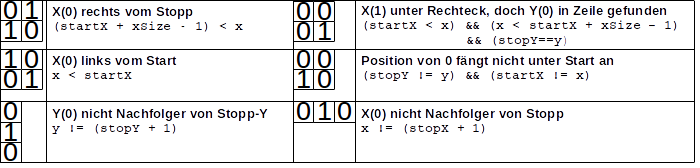
\includegraphics[scale=0.75]{mismatches.png}
    \caption{Ausschließende Bit-Muster mit Regeln}
    \label{fig:mismatches}
\end{figure}

Werden diese Muster nicht erkannt und schwarze Pixel existieren, dann existiert ein Rechteck (\texttt{FoundOne}). Andernfalls werden nicht zuzuordnende schwarze Pixel (\texttt{Mismatch}) oder gar keine schwarzen Pixel (\texttt{Nothing}) im Bild gefunden.

Nachdem jeder Prozess sein Teilbild bearbeitet hat, muss der \texttt{Master} alle Ergebnisse zusammenfassen. Zunächst sammelt der \texttt{Master} alle Teilergebnisse mit \texttt{MPI\_Gather} ein, danach bewertet er die Ergebnisse in folgenden Schritten.

\begin{enumerate}
	\item Gibt es ein Teilbild mit schwarzen Pixeln, welche aber kein Rechteck bilden, dann kann direkt abgebrochen werden mit \texttt{Mismatch}.
	\item Wenn alle Teilbilder \texttt{Nothing} finden kann ebenfalls abgebrochen werden mit \texttt{Nothing}.
	\item Gibt es nur ein \texttt{FoundOne} und sonst \texttt{Nothing}, kann das Rechteck ausgegeben werden.
\end{enumerate}

Falls mehrere \texttt{FoundOne} vorliegen und es wurde nicht abgebrochen, muss der \texttt{Master} überprüfen ob die gefundenen Rechtecke zusammenhängend sind.
Folgende Kriterien müssen für alle Prozesse, welche ein \texttt{FoundOne} liefern, überprüft werden.

\begin{enumerate}
	\item Die Start- und Stop-X Werte stimmen bei jedem Rechteck überein.
	\item Bis auf den ersten Prozess der ein Rechteck in einer Zeile gefunden hat, müssen alle Prozesse schwarze Pixel in ihrer ersten Zeile finden.
	\item Bis auf den letzten Prozess der ein Rechteck gefunden hat, müssen alle Prozesse schwarze Pixel in ihrer letzten Zeile finden.
\end{enumerate}

Nach dieser Überprüfung kann der Master-Prozess das Ergebnis ermitteln und die Start- und Stopp-Koordinaten des gefundenen Rechtecks ausgeben. 

Durch die Betrachtung der Umsetzung stellt man fest, dass für den sequentiellen Algorithmus ein Best-Case darin besteht sofort ein \texttt{Mismatch} zu finden, dadurch kann direkt abgebrochen werden. 
Der Average-Case stellt \texttt{Nothing} dar, da dass gesamte Digitalbild überprüft wird, aber keine weitere Auswertung der Rechteckmuster erfolgen muss.
Der Worst-Case besteht darin mehrere Rechtecke zu finden, welche auf Zusammengehörigkeit untersucht werden müssen.
Für die Untersuchungen zur Laufzeit werden diese drei Fälle berücksichtigt.

\subsection{Verwendung}
\subsubsection{Ausführung}
Der Quellcode kann mit Hilfe des folgenden Aufrufs kompiliert werden:

\begin{itemize}
	\item \texttt{cmake CMakeLists.txt -DCMAKE\_BUILD\_TYPE=RELEASE \&\& make}
\end{itemize}

Mif folgenden Befehl wird das Programm auf 4 Prozessoren ausgeführt:

\begin{itemize}
	\item \texttt{mpirun -npernode 4 rectanglePatternDetection} \textbf{FILE}
\end{itemize}

Für das Programm können Kommandozeilenargumente zur Angabe des Konfigurationsfiles zur Erstellung des zu untersuchenden Digitalbildes angegeben werden.

\subsubsection{Konfigurationsfile}
Die Anwendung unterstützt drei Modi zur Erzeugung des Digitalbildes, welcher dieser Modi verwendet wird, steht immer in der ersten Zeile des Files.
\paragraph{Modus 2: Custom Mode}Der \texttt{Custom Mode} ermöglicht die direkte Angabe einer $n*n$ Matrix aus Nullen und Einsen, diese wird ab Zeile Zwei zeilenweise angegeben.
\paragraph{Modus 1: Single Fields und Modus 0: Rectangle}
Um eine komfortable Eingabe zu realisieren, wird für die Modi 1 und 0 nicht die direkte Angabe der Matrix, sondern nur die Angabe einzelne Parameter realisiert.
Aus diesen Angaben wird dann das Digitalbild im Programm generiert.
Die zweite Zeile beschreibt die Größe $n$ und die Dritte die zu verwendende Hintergrundfarbe (0 oder 1). 
Aus diesen zwei Parametern kann im Programm leicht eine $n*n$ Matrix der angegebenen Hintergrundfarbe (0 oder 1) generiert werden.
Durch die vierte Zeile werden Koordinatenpaare in der Form: \texttt{x y} angegeben. Modus 1 interpretiert diese Koordinaten als einzelne Felder, welche im Bild umgedreht \linebreak ($0 \rightarrow 1,1 \rightarrow 0$) werden müssen. 
Modus 0 hingegen interpretiert nur die ersten drei Koordinatenpaare als Ortsvektoren der oberen Rechteck-Ecke, die das Rechteck aufspannen. 
Es ist notwendig, dass dabei die Reihenfolge: obere Ecke links, obere Ecke rechts und untere Ecke links eingehalten wird.
Durch die angegebenen Kodierungen (Modus 1 und 0) ist es möglich sehr große Digitalbilder mit der Anwendung zu testen, ohne dass diese tatsächlich  als physisch gespeicherte Dateien existieren müssen. 
Im Gegensatz dazu kann durch Modus 2 direkt die Matrix eingegeben werden, dieser Modus findet vorallem für kleinere $n$ Anwendung. 
Durch das Konfigurationsfile können somit sehr leicht Digitalbilder mit den vorher betrachteten Fällen \texttt{Nothing}, \texttt{Mitmatch} und \texttt{FoundOne} für kleine und große $n$ erzeugt werden. Im folgenden kann sieht man den Inhalt von Beispiel-Konfigurationsfiles.

\begin{figure}[htb]
    \centering
    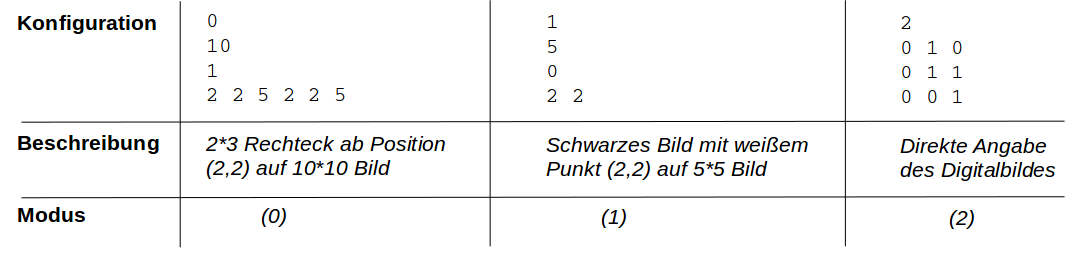
\includegraphics[scale=0.38]{configfiles.png}
    \caption{Beispiel-Konfigurationen für die Bilderstellung}
    \label{fig:configfiles}
\end{figure}

\subsection{Laufzeitverhalten}
Für die Untersuchungen des Laufzeitverhaltens werden im folgenden feste $n$ mit variierenden $p$ bis maximal 44 und feste $p$ mit variierende $n$ bis maximal 40000 betrachtet. Da das Maximum für das Quadratische Raster in etwa bei $n=45000$ liegt, können dennoch Aussagen über die Laufzeit getroffen werden. Das Maximum begründet sich an der Obergrenze der zu sendenden Datenpackete des Datentyps \texttt{MPI\_Short} über den Befehl \texttt{MPI\_Scatter}.
\begin{figure}[htb]
\begin{minipage}{0.49\textwidth}
\begin{tikzpicture}
\begin{axis}
[           scale=0.9,
            grid = major,
            grid style={dashed, gray!30},
            ylabel=Zeit in s,
            xlabel=n,
            legend style={at={(1.1,-0.1)}, anchor=north}
]
\addplot[red, mark=*] table [x=n, y=Mittel , col sep=space] {../rectangle/measures/nScaling/44/measure1.csv};
\addplot[blue, mark=+] table [x=n, y=Mittel , col sep=space] {../rectangle/measures/nScaling/44/measure2.csv};
\addplot[black, mark=x] table [x=n, y=Mittel , col sep=space] {../rectangle/measures/nScaling/44/measure0.csv};
\legend{FoundOne, Nothing,Mismatch}
\end{axis}
\end{tikzpicture}
	\caption{p = 44}
	\label{ref:p44}
\end{minipage}
\hfill
\begin{minipage}{0.49\textwidth}
\begin{tikzpicture}
\begin{axis}
[           scale=0.9,
            grid = major,
            grid style={dashed, gray!30},
            ylabel=Zeit in s,
            xlabel=n,
            legend style={at={(5.1,-0.1)}, anchor=north}
]
\addplot[red, mark=*] table [x=n, y=Mittel , col sep=space] {../rectangle/measures/nScaling/1/measure1.csv};
\addplot[blue, mark=+] table [x=n, y=Mittel , col sep=space] {../rectangle/measures/nScaling/1/measure2.csv};
\addplot[black, mark=x] table [x=n, y=Mittel , col sep=space] {../rectangle/measures/nScaling/1/measure0.csv};
\legend{FoundOne, Nothing,Mismatch}
\end{axis}
\end{tikzpicture}
	\caption{p = 1}
	\label{ref:p1}
\end{minipage}
\end{figure}
Wie man aus den gegebenen Laufzeitmessungen (\autoref{ref:p44} und \autoref{ref:p1}) für feste $p$ entnehmen kann, verschlechtert sich die Laufzeit beider Messungen quadratisch.
Dies ist mit dem Aufwand der Überprüfung des quadratischen Bildes zu begründen.
Für den sequentiellen Fall liefern alle drei Fälle: \texttt{Mismatch}, \texttt{FoundOne} und \texttt{Nothing} wesentlich kürzere Laufzeiten, als für den parallelen. 
Dies ist damit begründet, dass im sequentiellen Fall keine Kommunikation für die Auswertung notwendig ist, da der \texttt{Master} direkt seine Suche abbrechen kann. 
Im parallelem Fall muss der \texttt{Master} auf alle Teilergebnisse der anderen Prozessoren warten, hierbei entsteht durch das Senden und Empfangen ein Kommunikationsoverhead, welcher bei steigender Anzahl der verwendeten Prozessoren erhöht wird.
Außerdem ist zu beobachten, dass in \autoref{ref:p1} \texttt{Nothing} die Untergrenze darstellt und nicht \texttt{Mismatch}. Dies ist damit begründet, dass der \texttt{Mismatch} in den letzten Pixeln liegt\footnote{Für die Messungen wird ein \texttt{Mismatch} am Ende einer Zeile durch $0 1 0$ erzeugt.} und nicht eher abgebrochen werden kann, sondern immer alle $n*n$ Felder überprüft werden müssen. 
Neben dem bloßen Erkennen, ob es sich um weiße oder schwarze Pixel handelt, muss bei einem \texttt{Mismatch} wenigstens ein ausschließendes Muster von \autoref{fig:mismatches} überprüft worden sein.
Dieser Mehraufwand ist der Grund, weshalb \texttt{Mismatch} ein schlechteres Laufzeitverhalten als \texttt{Nothing} in \autoref{ref:p1} aufweist.
Ferner liefert \texttt{FoundOne} den Worst-Case für beide Messungen, da in beiden Fällen die ausschließenden Muster geprüft werden müssen. 
Durch die folgendenden Darstellungen (\autoref{ref:n10000} und \autoref{ref:n40000}) wird das Laufzeitverhalten für ein festes $n$ ersichtlich.
\begin{figure}[htb]
\begin{minipage}{0.49\textwidth}
\begin{tikzpicture}
\begin{axis}
[           scale=0.9,
            grid = major,
            grid style={dashed, gray!30},
            ylabel=Zeit in s,
            xlabel=p,
            legend style={at={(1.1,-0.1)}, anchor=north}
]
\addplot[red, mark=*] table [x=p, y=Mittel , col sep=space] {../rectangle/measures/processorScaling/44/10000/measure1.csv};
\addplot[blue, mark=+] table [x=p, y=Mittel,, col sep=space] {../rectangle/measures/processorScaling/44/10000/measure2.csv};
\addplot[black, mark=x] table [x=p, y=Mittel , col sep=space] {../rectangle/measures/processorScaling/44/10000/measure0.csv};
\legend{FoundOne, Nothing,Mismatch}
\end{axis}
\end{tikzpicture}
	\caption{n = 10000}
	\label{ref:n10000}
\end{minipage}
\hfill
\begin{minipage}{0.49\textwidth}
\begin{tikzpicture}
\begin{axis}
[           scale=0.9,
            grid = major,
            grid style={dashed, gray!30},
            ylabel=Zeit in s,
            xlabel=p,
            legend style={at={(5.1,-0.1)}, anchor=north}
]
\addplot[red, mark=*]  table [x=p, y=Mittel , col sep=space] {../rectangle/measures/processorScaling/44/40000/measure1.csv};
\addplot[blue, mark=+] table [x=p, y=Mittel,, col sep=space] {../rectangle/measures/processorScaling/44/40000/measure2.csv};
\addplot[black, mark=x] table [x=p, y=Mittel , col sep=space] {../rectangle/measures/processorScaling/44/40000/measure0.csv};
\legend{FoundOne, Nothing,Mismatch}
\end{axis}
\end{tikzpicture}
	\caption{n = 40000}
	\label{ref:n40000}
\end{minipage}
\end{figure}

Aus den Darstellungen kann man entnehmen, dass sich das Laufzeitverhalten für steigende $p$ logarithmisch verschlechtert. 
Das heißt für kleine $p$ ist der Anstieg der Laufzeit stets hoch, für große $p$ nimmt dieser Anstieg ab, bis die Laufzeit in Abhängigkeit von $p$ einer konstanten Funktion gleicht. 
Außerdem kann man erkennen, dass der sequentielle Fall wieder die besten Laufzeiten besitzt. 
Betrachtet man die unterschiedlichen Ergebnisse bildet \texttt{FoundOne} wieder den Worst-Case. 
Der Best-Case für $p=1$ kann diesmal durch \texttt{Mismatch} gezeigt werden, da ein vorzeitiger Abbruch durch das Vorkommen eines \texttt{Mismatches} in Zeile 4000 erreicht wird. 
Im parallelem Fall kann nicht eher abgebrochen werden, da erst alle Teilbilder durchsucht werden müssen, so dass ab einer Prozessorzahl von 2 \texttt{Nothing} und \texttt{Mismatch} das gleiche Laufzeitverhalten besitzen.
%TODO ab hier weiter lesen
\subsection{Speedup und Effizienz}
Die folgenden Abbildungen beziehen sich auf die Auswertungen zum Speedup und zur Effizienz. 
\begin{figure}[htb]
\begin{minipage}{0.49\textwidth}
\begin{tikzpicture}
\begin{axis}
[  			grid = major,
			scale=0.9,
            grid style={dashed, gray!30},
            ylabel=SpeedUp,
            xlabel=p,
            legend style={at={(1.1,-0.1)}, anchor=north}
]
\addplot[red, mark=*]  table [x=p, y=SpeedUp , col sep=space]{../rectangle/measures/processorScaling/44/40000/measure1.csv};
\addplot[blue, mark=*] table [x=p, y=SpeedUp , col sep=space]{../rectangle/measures/processorScaling/44/40000/measure2.csv};
\addplot[black, mark=*] table [x=p, y=SpeedUp , col sep=space]{../rectangle/measures/processorScaling/44/40000/measure0.csv};
\legend{FoundOne, Nothing,Mismatch}
\end{axis}
\end{tikzpicture}
	\caption{SpeedUp: n = 40000}
	\label{ref:speedUpn40000}
\end{minipage}
\hfill
\begin{minipage}{0.49\textwidth}
\begin{tikzpicture}
\begin{axis}
[  			grid = major,
			scale=0.9,
            grid style={dashed, gray!30},
            ylabel=SpeedUp,
            xlabel=p,
            legend style={at={(5.1,-0.1)}, anchor=north}
]
\addplot[red, mark=*]  table [x=p, y=SpeedUp , col sep=space]{../rectangle/measures/processorScaling/44/10000/measure1.csv};
\addplot[blue, mark=*] table [x=p, y=SpeedUp , col sep=space]{../rectangle/measures/processorScaling/44/10000/measure2.csv};
\addplot[black, mark=*] table [x=p, y=SpeedUp , col sep=space]{../rectangle/measures/processorScaling/44/10000/measure0.csv};
\legend{FoundOne, Nothing,Mismatch}
\end{axis}
\end{tikzpicture}
	\caption{SpeedUp: n = 10000}
	\label{ref:speedUpn10000}
\end{minipage}
\end{figure}

Wie schon bei der Untersuchung des Laufzeitverhaltens bemerkt wurde, verschlechtert sich die Laufzeit für den parallelen Fall enorm. 
Dieses Verhalten wird durch \autoref{ref:speedUpn10000} und \autoref{ref:speedUpn40000} bestätigt. 
Anstatt einen linearen Anstieg anzustreben, ähnelt die Funktion einer Hyperbel mit indirekter Proportionalität für alle Messungen. 
Mit steigenden $n$ müssen größere Teilbilder an alle Prozessoren kommuniziert werden, deshalb ist der Anstieg für $n=40000$ flacher als für $n=10000$, da der Kommunikationsoverhead stärker ins Gewicht fällt als die eigentliche Überprüfung. 
Außerdem erkennt man aus den Speedup-Darstellungen, die Abhängigkeit zu der sequentiellen Laufzeit. 
So dass der eigentliche Best-Case nun den schlechtesten Speedup aufweist, da der Referenzwert im sequentiellen Fall wesentlich geringer ist als die anderen Referenzwerte. 
Entsprechend verhält sich der Average-Case und Worst-Case. Folglich konnte gezeigt werden, dass die Problemstellung nicht geeignet ist für die Parallelisierung durch die anfallende Kommunikation. 

Im Anschluss wird näher auf die Effizienz eingegangen.
\begin{figure}[!ht]
\begin{minipage}{0.49\textwidth}
\begin{tikzpicture}
\begin{axis}
[  			grid = major,
			scale=0.9,
            grid style={dashed, gray!30},
            ylabel=Effizienz,
            xlabel=p,
            legend style={at={(1.1,-0.1)}, anchor=north}
]
\addplot[red, mark=*] table [x=p, y=Effizienz , col sep=space]{../rectangle/measures/processorScaling/44/40000/measure1.csv};
\addplot[blue, mark=*] table [x=p, y=Effizienz , col sep=space]{../rectangle/measures/processorScaling/44/40000/measure2.csv};
\addplot[black, mark=*] table [x=p, y=Effizienz , col sep=space]{../rectangle/measures/processorScaling/44/40000/measure0.csv};
\legend{FoundOne, Nothing,Mismatch}
\end{axis}
\end{tikzpicture}
	\caption{Effizienz: n = 40000}
	\label{ref:Effizienzn40000}
\end{minipage}
\hfill
\begin{minipage}{0.49\textwidth}
\begin{tikzpicture}
\begin{axis}
[  			grid = major,
			scale=0.9,
            grid style={dashed, gray!30},
            ylabel=Effizienz,
            xlabel=p,
            legend style={at={(5.1,-0.1)}, anchor=north}
]
\addplot[red, mark=*] table [x=p, y=Effizienz , col sep=space]{../rectangle/measures/processorScaling/44/10000/measure1.csv};
\addplot[blue, mark=*] table [x=p, y=Effizienz , col sep=space]{../rectangle/measures/processorScaling/44/10000/measure2.csv};
\addplot[black, mark=*] table [x=p, y=Effizienz , col sep=space]{../rectangle/measures/processorScaling/44/10000/measure0.csv};
\legend{FoundOne, Nothing,Mismatch}
\end{axis}
\end{tikzpicture}
	\caption{Effizienz: n = 10000}
	\label{ref:Effizienzn10000}
\end{minipage}
\end{figure}

Ähnlich zum Speedup weichen die Werte der Effizienz enorm zu einem gut parallelisierbaren Programm ab. 
Wie man durch die Darstellungen sieht sind alle Effizienzwerte für den parallelen Fall sehr gering (Effizienz von $0,2$\% bis $0,004$\%).
Hierdurch kann gezeigt werden, dass durch die Parallelisierung niemals eine Verbesserung erreicht wird. 
Außerdem erkennt man wie beim Speedup für größere $n$ (\autoref{ref:Effizienzn40000}) einen stärkeren Abfall als für kleinere $n$.
Dies ist wieder durch den stärker ins Gewicht fallenden Kommunikationsoverhead zu begründen.

\subsection{Fazit}
Die Problemstellung eine Rechteckmustererkennung umzusetzen und zu parallelisieren konnte erfolgreich, wie in \autoref{ref:realisierungRect} beschrieben, umgesetzt werden. 
Laufzeitmessungen ergaben, dass eine sequentielle Erkennung einer parallelen vorzuziehen ist.
Begründet ist diese starke Verschlechterung durch den anfallenden Kommunikationsoverhead und der zusätzlich notwendigen Auswertung der Teilergebnisse. 
Außerdem gibt es für die sequentielle Suche die Möglichkeit vorzeitig abzubrechen.
Anders als im parallelen Fall, da jeder Prozess sein Teilbild entsprechend durchsuchen muss.
Durch die Untersuchungen von variierenden $n$ konnte gezeigt werden, dass sich die Laufzeit quadratisch mit steigenden $n$ verschlechtert für alle $p$.
Folglich verschlechtert sich mit steigendem $n$ die Laufzeit des parallelen Programmes noch mehr.
Da sehr geringe Werte für Speedup und Effizienz ermittelt worden, wurde bewiesen, dass die Problemstellung sich nicht für die Parallelisierung eignet.
Folglich wird für die Erkennung von Rechteckmustern die sequentielle Variante empfohlen.

\pagebreak
\section{Projektaufgabe 2: Numerische Integration mittels Parabelformel}
\lstset{language=Fortran,frame=none, keepspaces=false,tabsize=1,captionpos=b, basicstyle=\scriptsize,showstringspaces=false,breaklines=true}  
In diesem Abschnitt wird auf die Projektaufgabe 2 eingegangen.
Zunächst wird kurz erklärt wie das Programm kompiliert und gestartet wird sowie auf die Kommandozeilenargumente eingegangen.
Im Anschluss wird die Realisierung und damit die Lösung des Problems betrachtet.
Anschließend erfolgt die Auswertung und im letzten Abschnitt wird ein Fazit gezogen.

\subsection{Verwendung}
\label{ref:verwendung}
Der Quellcode kann mit dem Aufruf von \texttt{1} auf dem MC-3-System kompiliert und mit \texttt{2} ausgeführt werden:
\begin{itemize}
	\item[1.] f77.px -o A2star.px A2star.f
	\item[2.] run -f0 4 2 A2star.px \textbf{FUNCTION} \textbf{N}
\end{itemize}
Für das Programm können Kommandozeilenargumente zur Auswahl der Testfunktion und die Größe der zu berechnenden Teilstücke des Integrals angegeben werden.
\paragraph{FUNCTION:}
Das Programmargument \textbf{FUNCTION} entscheidet darüber, welche der beiden gegebenen Testfunktionen verwendet wird.
Als gültige Eingabe wird \texttt{1} für Funktion 1 und \texttt{2} für Funktion 2 erwartet.
\paragraph{N:}
Das zweite Programmargument \textbf{N} gibt die 2er Potenz der zu berechnenden Teilstücke des Integrals an.
Je größer das \textbf{N} umso genauer wird das berechnete PI.
De höchstmöglichste zulässige Eingabe ist 20, dass sind 1048576 zu berechnende Teilstücke.
Diese Vorgehensweise soll zum Einen sicher stellen, dass \textbf{N} stets durch 2 Teilbar ist und zum Anderen das Laufzeitmessen vereinfachen, da ein exponentielles Wachstum vorliegt.
Sollte kein Programmargument angeben werden, so wird intern die Funktion 1 mit $n = 2^{15} = 32768$ verwendet.

Weiterhin muss die Divison von \textbf{n} durch Prozessorzahl ganzahlig sein, damit stets gewährleistet ist, dass die zu berechnende Anzahl an Teilstücke pro Prozessor eine ganzzahlige ist.

\subsection{Realisierung}
\label{ref:realisierung}
Grundlegend wurde sich bei der Realisierung für eine Stern-Topologie entschieden.
Gewählt wurde diese Topologie, da bei der Parallelisierung dieser Aufgabe ein Master existert, welche alle Teilergebnisse empfängt und summiert.
Weiterhin wurde diese Topologie bereits in einem Seminar implementiert.

Bedingt durch die Realisierung als Kommandozeilenparameter, entfällt der Kommunikationsoverhead für das Verteilen von \textbf{N} und \textbf{FUNCTION}.
Daher kennen alle Prozessoren \textbf{N} sowie die Testfunktion beim Programmstart.

Die Prozessoren können explizit ihre eigenen Bereich für die Teilstücke bestimmen und somit die numerische Berechnung durchführen.
Nach Abschluss der Berechnungen werden diese an den Master-Prozessor gesendet.
Der Master-Prozessor summiert die Ergebnisse der anderen Prozessoren zu seinem eigenem Ergebnis auf und wendet die Multiplikation $\frac{\textbf{h}}{3}$ auf das Ergebnis an.
Im Anschluss werden die Ergebnisse wie \texttt{Referenzwert-PI}, \texttt{Berechnetes-PI}, \texttt{Abweichung} und \texttt{Laufzeit} (nicht in Abbildung dargestellt) ausgegeben. 
Die \autoref{ref:main} zeigt dies.
\begin{figure}[h]
\hrulefill

\begin{minipage}{0.49\textwidth}
\begin{lstlisting}
	call startIntegration(f,n,integral,h)
	if(id.eq.0) then
		summe = integral
		do i=1,(np-1)
			call recv(topid,links(i),integral,8)
			summe = summe + integral
		enddo
		summe = h/3 * summe
	else
		call send(topid, link,integral,8)
	endif
\end{lstlisting}
	\caption{Empfangen und Auswerten}
	\label{ref:main}
\end{minipage}
\hfill
\vline
\begin{minipage}{0.49\textwidth}
\begin{lstlisting}
	nL = n / nprocs()
	aL = a + id * nL * h
	bL = aL + nL * h
	summe = getVal(f,aL) + getVal(f,bL)   
	step = aL + h
	do i=1,nL-1
		factor=2**(mod(i,2) + 1)
		summe = summe + (dble(getVal(f,step) * factor)
		step = step + h    
	enddo
\end{lstlisting}
	\caption{Berechnung der Teilstück}
	\label{ref:intervall}
\end{minipage}

\hrulefill
\end{figure}

Die numerische Berechnung des Integrals wird durch jeden Prozessor ausgeführt, aber jeder Prozessor führt nur einen Teil der kompletten Berechnung aus.
Die eigentliche Berechnung ist in der \autoref{ref:intervall} zu sehen.
Zunächst berechnet jeder Prozessor die Anzahl der durchzuführenden Berechnungen als lokales \textbf{n} (\textbf{nL}).
Im Anschluss werden Startwert (\textbf{aL}) und Endwert (\textbf{bL}) ermittelt.
Die Funktionswerte von \textbf{aL} und \textbf{bL} der Testfunktion werden addiert und in einer Summe gespeichert.
Im Anschluss werden die Zwischenstücke mit entsprechendem Faktor berechnet und ebenfalls summiert.
Die Variable \textbf{h} gibt dabei die allgemeine Schrittweite an und \textbf{step} den derzeitigen Schrittwert.

Nach erfolgter Berechnung sendet jeder Prozessor sein Ergebnis an den Master (falls der Prozessor nicht selbst der Master ist)

\subsection{Ergebnisse der Testfunktionen}
In diesem Unterabschnitt wird auf die erzielten Ergebnisse der Testfunktion 1 und 2 hinsichtlich ihrer Näherung zu Pi eingegangen.
Als Referenzwert für die Testunfktionen wurde Pi mit \textbf{3.141592653589793} verwendet.
Angemerkt sei, dass die Prozessoranzahl 6 ausgeschlossen wurde, da dadurch bei Division durch die 2er Potenz von \textbf{n} ein nicht ganzzahliges lokales \textbf{n} enstehen würde.
Durch das lokale \textbf{n}, würde zwar ein Näherungswert zu Pi bestimmt, aber dieses besitzt eine deutlich größere Abweichungen im Vergleich zu einer korrekten Eingabe.
Deswegen wird beim Programmstart diese Eingabe überprüft und gegebenenfalls bei falscher Eingabe das Programm beendet.

Die \autoref{ref:piP} zeigt die Abweichung zum Referenzwert von Pi bei einer konstanten Prozessoranzahl von 8 und einem sich verändernden \textbf{n}.
Wie in der Tabelle zu sehen ist liefert die Testfunktion 2 bessere Näherungswerte als Funktion 1.
Ein Grund dafür, dass die Funktion 1 schlechte Näherungswerte liefert, liegt unter Anderem an der Oberegrenze.
Diese Obergrenze ist Pi selbst.
Zusätzlich sind in der Funktion 1 die Schrittweiten bedeutend größer, als bei der Funktion 2.
Deswegen benötigt die Funktion ein größeres \textbf{n} um mehr Teilstücke berechnen zu können und somit ein genaueres Ergebnis zu liefern.
\begin{figure}[h]
\begin{minipage}{0.45\textwidth}
	\pgfplotstabletypeset[col sep=space
	,use comma
	,every head row/.style={before row={\hline},after row=\hline}
	,every last row/.style={after row=\hline}
	,every even column/.style={column type/.add={|}{|}}
	,columns={n,Abweichung-F1,Abweichung-F2}
	]{../integration/functionDiffp8.csv}
	\caption{Mit 8 Prozessoren}
	\label{ref:piP}
\end{minipage}
\hfill
\begin{minipage}{0.45\textwidth}
	\pgfplotstabletypeset[col sep=space
	,every head row/.style={before row={\hline},after row=\hline}
	,every last row/.style={after row=\hline}
	,every even column/.style={column type/.add={|}{|}}
	,columns={p,Abweichung-F1,Abweichung-F2}
	]{../integration/functionDiffn.csv}
	\caption{Mit n = 32768}
	\label{ref:piN}
\end{minipage}
\end{figure}
Die \autoref{ref:piN} zeigt ebenfalls die Abweichung, aber hier wird ein konstantes \textbf{n} von 32768 verwendet und die Prozessoranzahl variiert.
Das die Näherungswerte sich in Abhängigkeit von der verwendeten Prozessorzahl unterscheiden ist damit begründet, dass die Parabelformel mittlere Teilstücke mit einem Faktor von 4 beziehungsweise 2 wichtet.

\subsection{Laufzeitverhalten}
Im vorherigen Abschnitt wurden die Ergebnisse der Testfunktionen hinsichtlich Pi untersucht und nun wird eine Betrachtung hinsichtlich der Laufzeit durchgeführt.

Wie in der \autoref{ref:Laufzeitn} zu sehen ist lohnt sich für diese Aufgabenstellung eine Parallelisierung.
Mit steigendem \textbf{p} verringert sich die Laufzeit im Vergleich zum sequenziellen Fall.
Es ist zu vermuten das mit steigendem \textbf{p} der Laufzeitgewinn immer schwächer wird und ab einem gewissen Punkt wieder eine Laufzeitverschlechterung eintritt.
Begründet ist dies mit steigendem Kommukationsoverhead bei einer steigendem Prozessoranzahl.
Bei der hier verwendeten geringen Anzahl an Prozessoren mit einem Maximum von 8, spielt der Kommunikationsoverhead eine eher untergeordnete Rolle.
Zusätzlich ist zu sehen, dass die Testfunktion 1 langsamer ist als die Testfunktion 2.
Der Grund für diesen Laufzeitunterschied ist die Tatsache, dass die Berechnung von Sinus in Funktion 1 aufwändiger ist als die Division in Funktion 2.
\begin{figure}[h]
\begin{minipage}{0.49\textwidth}
\begin{tikzpicture}
\begin{axis}
[   		scale=0.9,
            grid = major,
            grid style={dashed, gray!30},
            ylabel=Zeit in s,
            xlabel=p,
            legend style={at={(1.1,-0.1)}, anchor=north}
]
\addplot[red, mark=*] table [x=p, y=T15 , col sep=space]{../integration/speedUpF1.csv};
\addplot[blue, mark=x] table [x=p, y=T15 , col sep=space]{../integration/speedUpF2.csv};
\legend{Funktion 1, Funktion 2}
\end{axis}
\end{tikzpicture}
	\caption{Laufzeit mit n = 32768}
	\label{ref:Laufzeitn}
\end{minipage}
\hfill
\begin{minipage}{0.49\textwidth}
\begin{tikzpicture}
\begin{axis}
[   		scale=0.9,
            grid = major,
            grid style={dashed, gray!30},
            ylabel=Zeit in s,
            xlabel=n,
            legend style={at={(5.1,-0.1)}, anchor=north}
]
\addplot[red, mark=*] table [x=n, y=T , col sep=space]{../integration/pConstF1.csv};
\addplot[blue, mark=x] table [x=n, y=T , col sep=space]{../integration/pConstF2.csv};
\legend{Funktion 1, Funktion 2}
\end{axis}
\end{tikzpicture}
	\caption{Laufzeit mit p = 8}
	\label{ref:LaufzeitP}
\end{minipage}
\end{figure}

Wie in der \autoref{ref:LaufzeitP} zu sehen ist steigt mit wachsendem \textbf{n} und konstantem \textbf{p} die Laufzeit beider Algorithmen an.
Es ist festzustellen, dass die Testfunktion 1 dabei einen stärkeren Anstieg aufweißt als Testfunktion 2.
Die Ergebnisse entsprechen dem erwarteten Verhalten, denn mit steigendem \textbf{n} sollte bei diesem Problem die Laufzeit linear steigen.

\subsection{Speedup und Effizienz}
In diesem Abschnitt sollen nun Speedup und Effizienz für die Testfunktionen 1 und 2 betrachtet werden.

In der \autoref{ref:speedF1} ist der ermittelte Speedup für die Tesfunktion 1 mit zwei verschieden Werten für \textbf{n} zu sehen.
Bei einem großem \textbf{n} ist zu sehen, dass ein deutlich besserer Speedup erzielt wird, als bei einem kleineren \textbf{n}.
Dieses Verhalten wird auch in der Funktion 2 nachgewiesen, wie man in der \autoref{ref:speedF2} sehen kann.
Bei einem kleinen \textbf{n} flacht der Speedup bedeutend schneller ab.
Bedingt ist dies dadurch, dass bei einem kleineren \textbf{n} die Berechnung der Integralstücke sehr schnell erfolgt und die Laufzeit für die Kommunikation und Summation markanter in die Laufzeitermittlung eingeht.
Dennoch lässt sich sagen, dass bei dieser Aufgabe bei maximal 8 Prozessoren ein sehr guter Speedup erreicht wird.
Die parallele Ausführung der Funktion 1 zeigt eine stärkere Verbesserung als Funktion 2. 
Es wird vermutet, dass die Parallelisierung der langsameren Sinusfunktion eine stärkere Verbesserung der Laufzeit erzielt, als sie bei der schnelleren Division erzielen kann.
Deshalb ist der Speedup von Funktion 2 schlechter als von Funktion 1.
\begin{figure}[h]
\begin{minipage}{0.49\textwidth}
\begin{tikzpicture}
\begin{axis}
[ 
           	grid = major,
			scale = 0.9,
            grid style={dashed, gray!30},
            ylabel=SpeedUp,
            xlabel=p,
            legend style={at={(1.1,-0.1)}, anchor=north}
]
\addplot[red, mark=*] table [x=p, y=SpeedUp15 , col sep=space]{../integration/speedUpF1.csv};
\addplot[blue, mark=x] table [x=p, y=SpeedUp12 , col sep=space]{../integration/speedUpF1.csv};
\addplot[black] table [x=p, y=IdealSpeedUp, col sep=space]{../integration/speedUpF1.csv};
\legend{n = 32768,n = 4096, Ideal}
\end{axis}
\end{tikzpicture}
	\caption{SpeedUp Funktion 1}
	\label{ref:speedF1}
\end{minipage}
\hfill
\begin{minipage}{0.49\textwidth}
\begin{tikzpicture}
\begin{axis}
[  			grid = major,
			scale = 0.9,
            grid style={dashed, gray!30},
            ylabel=SpeedUp,
            xlabel=p,
            legend style={at={(5.1,-0.1)}, anchor=north}
]
\addplot[red, mark=*] table [x=p, y=SpeedUp15 , col sep=space]{../integration/speedUpF2.csv};
\addplot[blue, mark=x] table [x=p, y=SpeedUp12 , col sep=space]{../integration/speedUpF2.csv};
\addplot[black] table [x=p, y=IdealSpeedUp, col sep=space]{../integration/speedUpF2.csv};
\legend{n = 32768,n = 4096,Ideal}
\end{axis}
\end{tikzpicture}
	\caption{SpeedUp Funktion 2}
	\label{ref:speedF2}
\end{minipage}
\end{figure}
Im folgenden werden die Funktionen hinsichtlich ihrer Effizienz betrachtet.
In der \autoref{ref:EffizienzF1} und \autoref{ref:EffizienzF2} ist die Effizienz für die Funktion 1 sowie 2 dargestellt.
Aufgrund das bei einem großen \textbf{n} ein besserer Speedup erzielt wird, werden bei Funktion 1 und 2 relativ hohe Effizienzwerte erreicht.
Es ist außerdem zu sehen, dass Funktion 1 im Allgemeinen effizienter ist als Funktion 2.
Außerdem wird die höchste Effizienz bei der Parallelisierung mit 2 Prozessoren erreicht.
Dies gilt für Funktion 1 und Funktion 2 gleichermaßen.
Bei einem kleineren \textbf{n} sinkt die Effizienz bedeutend schneller als bei einem großen, wobei auch hier Funktion 1 im Allgemeinen besser ist.
\begin{figure}[h]
\begin{minipage}{0.49\textwidth}
\begin{tikzpicture}
\begin{axis}
[   		scale=0.9,
            grid = major,
            grid style={dashed, gray!30},
            ylabel=Effizienz,
            xlabel=p,
            legend style={at={(1.1,-0.1)}, anchor=north}
]
\addplot[red, mark=*] table [x=p, y=Effizienz15 , col sep=space]{../integration/speedUpF1.csv};
\addplot[blue, mark=x] table [x=p, y=Effizienz12 , col sep=space]{../integration/speedUpF1.csv};
\addplot[black] table [x=p, y=IdealEffizienz, col sep=space]{../integration/speedUpF1.csv};
\legend{n = 32768,n = 4096}
\end{axis}
\end{tikzpicture}
	\caption{Effizienz Funktion 1}
	\label{ref:EffizienzF1}
\end{minipage}
\hfill
\begin{minipage}{0.49\textwidth}
\begin{tikzpicture}
\begin{axis}
[   		scale=0.9,
            grid = major,
            grid style={dashed, gray!30},
            ylabel=Effizienz,
            xlabel=p,
            legend style={at={(5.1,-0.1)}, anchor=north}
]
\addplot[red, mark=*] table [x=p, y=Effizienz15 , col sep=space]{../integration/speedUpF2.csv};
\addplot[blue, mark=x] table [x=p, y=Effizienz12 , col sep=space]{../integration/speedUpF2.csv};
\addplot[black] table [x=p, y=IdealEffizienz, col sep=space]{../integration/speedUpF2.csv};
\legend{n = 32768,n = 4096}
\end{axis}
\end{tikzpicture}
	\caption{Effizienz Funktion 2}
	\label{ref:EffizienzF2}
\end{minipage}
\end{figure}
\subsection{Fazit}
\label{ref:fazit}
Die Problemstellung der numerischen Integration mittels Parabelformel konnte erfolgreich in Fortran umgesetzt werden.
Laufzeitmessungen sowie Betrachtung von Speedup und Effizienz ergaben, dass eine Parallelisierung für diese Aufgabenstellung sehr geeignet ist.
Aufgrund des geringen Kommunikationsoverhead fällt dieser bei der geringen Prozessoranzahl ($\textbf{p} \le 8$) kaum ins Gewicht, falls das \textbf{n} ausreichend groß ist.
Dies liegt daran, dass die Laufzeit für Kommunikation und Summation im Vergleich zur Berechnung stärker ins Gewicht fällt.

Zusätzlich ist festzuhalten, dass die Funktion 2 bessere Näherungswerte für Pi liefert als die Funktion 1.
Obwohl die Funktion 2 ein besseres Laufzeitverhalten als Funktion 1 besitzt ist Funktion 1 doch etwas effizienter bei der Parallelisierung.
Denn die Funktion 2 ist bereits sehr schnell und erreicht durch die Parallisierung einen flachereren Anstieg der Laufzeit als Funktion 1.
Der Gewinn der Parallelisierung ist folglich für Funktion 1 größer.
Es wird dennoch empfohlen Funktion 2 zu verwenden, aufgrund der besseren Näherungswerte für ein kleines \textbf{n} und der Allgemeinen besseren Laufzeit.

\end{document}
